\section{The role of width}

\label{2305:sec:width}
Thus far our discussion has focused on the well-specified case. We now discuss the role of width in escaping mediocrity. Our starting point are the deterministic ODEs \eqref{2305:eq:overlapping_ODE} for the sufficient statistics derived in Section \ref{2305:sec:odes}. As in our previous analysis, we focus on the spherical setting where $w_{i}\in\mathbb{S}^{d-1}(\sqrt{d})$, implying $Q_{jj}=1$, see Appendix \ref{2305:app:spherical_constraint} for a detailed derivation. First, we derive analytical expressions for the exit time for arbitrary width $p\geq 1$ in the particular case where the second layer is fixed at initialization $a^{0}_{j}=1$, $\forall j\in[p]$. The role played by the second layer is then discussed in Subsection \ref{2305:subsec:second_layer}.

Differently from the $p=1$ case, the process cannot be described by a single sufficient statistic, and instead we have to track \(\sfrac{p(p-1)}{2}\) non-diagonal entries of \(\Q\) (it is a symmetric matrix), and \(p\) components of the vector \(\M\). Note that equation \eqref{2305:eq:exit_time_implicit_equation} remains valid to define \(t_\text{ext}\), and can be solved numerically. An analytical expression for the exit time can be derived under similar assumptions to the ones discussed in Section \ref{2305:sec:exit:deterministic}, although the derivation is significantly more cumbersome. Full details can be found in Appendix ~\ref{2305:app:exit_time-derivation}. The final expressions for the annealed and quenched exit times are given by
\begin{align}
    \label{2305:eq:exit_time:p_annealed}
    t_\text{ext}^\text{(anl)} =& \frac{\log\left[\frac{T(p+1)d+(p+1)(1-T)}{2 p}\right]}{8\left[
      1 -\frac{\gamma}{p} \left(1 +\frac{1}{p} + \frac{4}{p^2} + \frac\Delta2 \right)
    \right]}, \\
    \label{2305:eq:exit_time:p_quenched}
    t_\text{ext}^\text{(qnc)} =& \mathbb E_{\mu_0,\tau_0 \sim \mathcal{P}^d_p} \left[
        \frac{\log\left[\frac{Tp(p+1)d+(2\mu_0p-\tau_0)(1-T)}{2\mu_0 p}\right]}{8\left[
      1 -\frac{\gamma}{p} \left(1 +\frac{1}{p} + \frac{4}{p^2} + \frac\Delta2 \right)
    \right]}
    \right].
\end{align}
With the distribution of the variables \(\tau_0\) and \(\mu_0\) given by
\[
    \mu_0,\tau_0 \sim \mathcal{P}^d_p \quad\text{where }
    \mathcal{P}^d_p \equiv \left(d\sum_{j=1}^{p}(u_j\cdot v)^2, 2d\sum_{j=1}^{p}\sum_{l=j+1}^{p}(u_j\cdot u_l)^2\right)\text{ with } v,u_j\sim\mathbb S^{d-1}(1).
\]



Notice that $t_\text{ext}$ is a monotonically decreasing function of the width. Nevertheless, for any $p\geq 1$, the leading order dependence in the dimension is $t_\text{ext} = \log{d}$. Hence, despite helping to escape mediocrity, increasing the width cannot mitigate it. This can be contrasted to other aspects in which overparameterization can significantly help optimization, for instance with global convergence \citep{bach2022gradient}. Interestingly, the minimal escaping time \[t_\text{ext}^\text{(anl)} = \frac{1}{4}\log(\frac{T(p+1)d+(p+1)(1-T)}{2p})\], obtained by choosing the learning rate that minimizes the sample complexity for escaping, has the same pre-factor for any width $p\geq 1$, with the only differences being the dependence in $p$ inside the logarithm and in the time scaling \(t=\sfrac{\nu\gamma}{pd}\). At infinite width $p\to\infty$, this simply amounts to a factor $\frac{12+\Delta}{2+\Delta}$ with respect to $p=1$. Details of this computation can be found in Appendix~\ref{2305:app:overp_gain}.

% \begin{figure}
\begin{figure}
    \centering        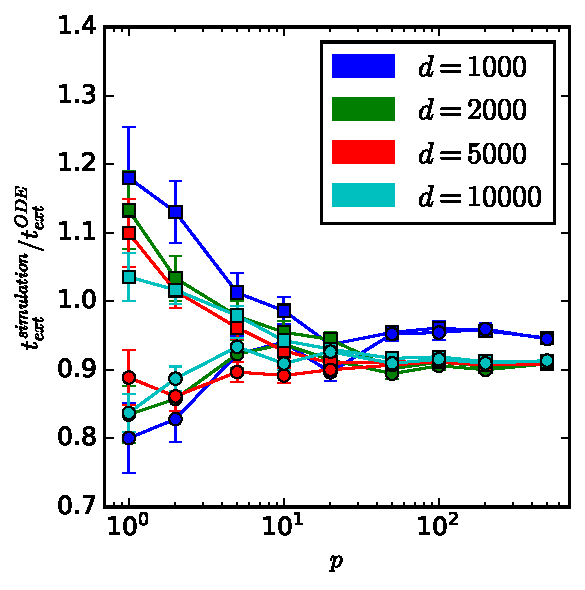
\includegraphics[width=0.49\textwidth]{figs/ode-exittimes-rateos}
    \caption{Ratio between the measured \(t_\text{ext}\) from simulations and the corresponding analytical formula (square = annealed, circle = quenched). We average over many initial conditions, for different values of \(p\). The ratio \(\sfrac{\gamma}{p}\) has been kept constant for different simulations.}
    \label{2305:fig:different_width_exit_times}
    % 
\end{figure}
% \end{figure}

Figure~\ref{2305:fig:different_width_exit_times} compares our analytical formulas \eqref{2305:eq:exit_time:p_annealed} and \eqref{2305:eq:exit_time:p_quenched} with real one-pass SGD simulations. The simulation are averaged over many different instances of the initial conditions, and the ratio \(\sfrac{\gamma}{p}\) is kept constant when varying \(p\), for not having discrepancies due to the different learning rate scaling. It's interesting to notice how the two different formulas gives the same outcome for large width \(p\gg1\). Moreover, for narrow networks they essentially differ from by a $d$ independent constant. Figure~\ref{2305:fig:different_width_exit_times} also suggests that, as for $p=1$, the stochasticity can be neglected in the estimation of the exit time. In Appendix~\ref{2305:app:SDE_with_generic_width} we provide further evidence of that. 

\subsection{Training the second layer}\label{2305:subsec:second_layer}

In the previous section, we have derived analytical expressions for the exit time in the particular case of fixed second layer weights $a^{0}_{j}=1$. Here, we provide numerical evidence that training the second layer does not significantly change our conclusions.

The key challenge is that by training the second layer we can't measure \(t_\text{ext}\) as the time needed to escape the risk at initialization. Indeed, from equation  \eqref{2305:eq:exit_time_implicit_equation} it can be seen that in the very first steps of the learning the vector \(a\) changes slightly to adapt to the initial conditions, thereby fitting the noise. In this scenario, instead of looking directly at the risk, we can instead use the largest component of the correlation vector \(m\) as a measure on how much the network has learned. At random initialization, this is of order \(\sfrac{1}{\sqrt{d}}\), grows to $1$ as the neural network correlates with the target weights. A natural choice for initializing the second layer weights is $a^0_j = 1$,  $\forall j \in [p]$. In principle, this initial condition guarantees that the risk at initialization is exactly equal to the case where \(a_j\) is fixed. On the other hand, as we already point out, the initial plateau where the dynamics gets stuck depends on the particular second layer initial condition. Even for other choices of initialization, e.g. \(a_j \sim \text{Bernoulli}(\sfrac12)\), the dynamics quickly goes a plateau, so it does not really matter which \(a_j^0\) is used. Therefore, for simplicity we choose a homogeneous initialization \(a^0_j = 1\). Figure~\ref{2305:fig:second_layer} compares the evolution of the maximum correlation when learning the second layer or not, for different values of \(p\). 

It is important to stress that we are not claiming that the time needed to reach the minimum of the population risk is the same when training or not the second layer, as can be seen in Fig.~\ref{2305:fig:second_layer}. Instead, our result highlights that the time needed to escape the flat directions at initialization are close. In fact, after the two layer neural network has escaped mediocrity, the dynamics can be very different whether the second layer weights are trained or not. For instance, \(a\) could become sparse with just a few neurons contributes to the output, or it could remain close to homogeneous \(a_j=1\), and with all neurons correlating with the target. Although studying the dynamics after escaping mediocrity is surely an interesting endeavor, it's out of the scope of this manuscript. 

\begin{figure}
    \centering
    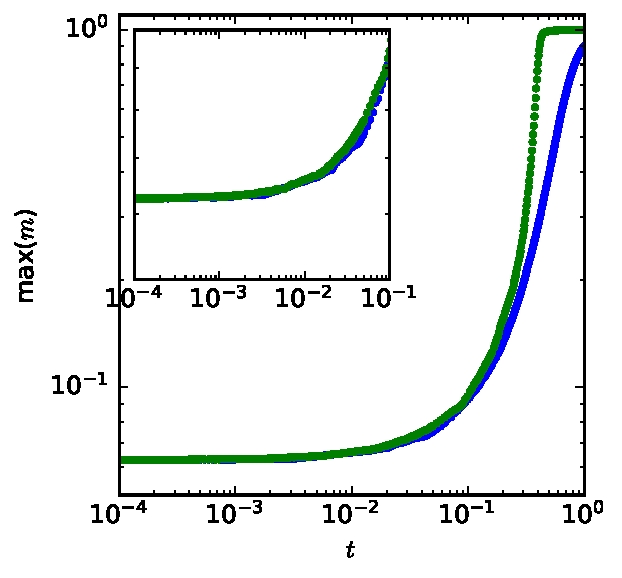
\includegraphics[width=.49\textwidth]{figs/twolayer-p20}
    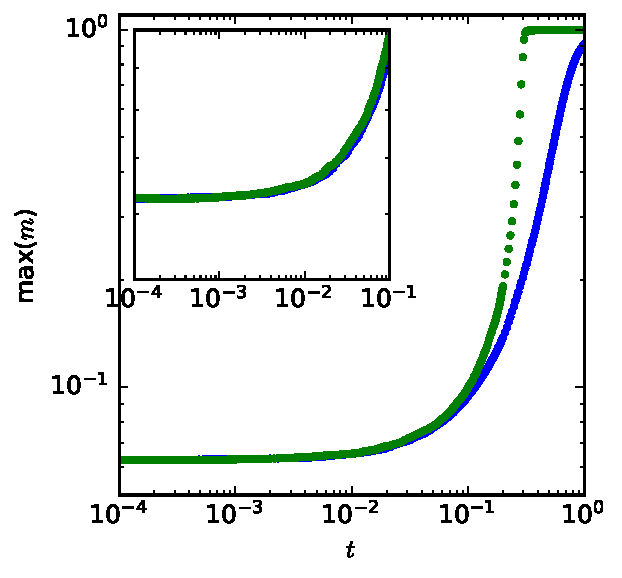
\includegraphics[width=.49\textwidth]{figs/twolayer-p50}
    \caption{\(p=20\) (left), \(p=50\) (right), \(d = 1000\). Comparison between the growth of \(\max{m}\) throughout the learning process, when the second layer is fixed (blue) and trained (green). The dynamics is obviously different far from the starting point, but when we zoom close to the exit point, the two processes have the same behavior, \(t_\text{ext}\) included.}
    \label{2305:fig:second_layer}
\end{figure}

